\documentclass[20pt,landscape]{foils}
\usepackage[portuges,english,german]{babel}
\usepackage{amssymb}
\usepackage{verbatim}
\usepackage{subfigure}
\usepackage{pdf14}
\usepackage{animate}

%--------------------------------------------------
%   ppower4 slides
%   acroread slides.pp4
\usepackage[pdftex]{color}
\newcommand{\figs}{figures}
%--------------------------------------------------
\usepackage{lastpage}
\usepackage[nomarkers]{pause}
\usepackage[pdftex]{geometry}
%\usepackage[margin=0.2in, pdftex]{geometry}
\usepackage[pdftex]{graphicx}
\usepackage[utf8]{inputenc}
\usepackage{fancybox}
\usepackage{background}
\usepackage{pp4slide} 
\usepackage{alltt}
\usepackage{pause}
\usepackage{shadow}
\usepackage{mpmulti}
\usepackage{pifont}
\usepackage{multirow}
\usepackage{subfigure}
\usepackage{wrapfig}
\geometry{headsep=3ex,hscale=0.9,vscale=0.8}
\DeclareGraphicsExtensions{.pdf,.eps,.ps}
\definecolor{bgmag}{rgb}{0.92,0.92,0.92}
\definecolor{pausecolor}{rgb}{1,1,1}
\definecolor{normalcolor}{rgb}{0,0,0}
\definecolor{highlightcolor}{rgb}{0.1,0.2,1}
\definecolor{myblue}{rgb}{0.1,0.2,1}
\definecolor{myblack}{rgb}{0.5,0.5,0.5}
\definecolor{myred}{rgb}{1,0.3,0}
\pagecolor{bgmag}
\color{black}

\newcommand{\normaltext}{\textcolor{normalcolor}}
\newcommand{\redtext}[1]{\textcolor{myred}{\bf #1}}
\newcommand{\yellowtext}[1]{\textcolor{highlightcolor}{\bf #1}} %% this is blue
\newcommand{\code}[1]{\texttt{#1}}
\newcommand{\redcode}{\textcolor{myred}}
\newcommand{\yellowcode}{\textcolor{yellow}}
\newcommand{\bluetext}{\textcolor{myblue}}

\newcommand{\titulo}[1]{\foilhead{\textcolor{highlightcolor}{\Large{\bf #1}}\vspace{-1cm}}}

\newenvironment{lista}{
  \renewcommand{\labelitemi}{\redtext{\ding{228}}}
  \vspace{-0.5cm}
  \begin{itemize}
    \setlength{\itemsep}{0mm}
}{\end{itemize}}

\newenvironment{sublista}{
\renewcommand{\labelitemii}{\redtext{\ding{169}}}
\begin{itemize}
\setlength{\itemsep}{0mm}
}{\end{itemize}}

\newenvironment{codigo}{
\begin{alltt}
\renewcommand{\baselinestretch}{0.8}
}{\end{alltt}}

\newcounter{pausecount}
\def\mypause{\pauselevel{build\space=\arabic{pausecount}\space:\arabic{pausecount}}\pause\addtocounter{pausecount}{1}}

\pausecolors{pausecolor}{normalcolor}{highlightcolor}
\leftheader{\textcolor{myblack} {On Extending a Full-Sharing
    Multithreaded Tabling Design with Batched Scheduling}}

\rightheader{\textcolor{myblack}{Miguel Areias and Ricardo Rocha}}
\Restriction{\textcolor{myblack}{
\includegraphics[scale=0.30]{figures/slate.pdf}}} 

\rightfooter{\textcolor{myblack}{{\bf \thepage ~/~\pageref{LastPage}}}}

%--------------------------------------------------

\title{\textcolor{blue}{\LARGE On Extending a Full-Sharing 
    \\\vspace{0.5cm} Multithreaded Tabling Design \\\vspace{0.5cm}
    with Batched
    Scheduling\vspace{0.2cm}}}

\author{Miguel Areias and Ricardo Rocha\\
CRACS $\&$ INESC-TEC LA\\
Faculty of Sciences, University of Porto, Portugal\\ 
\emph{miguel-areias@dcc.fc.up.pt \hspace{1cm} ricroc@dcc.fc.up.pt} \\ \\
  Yap Prolog: \textit{ http://www.dcc.fc.up.pt/$\sim$vsc/Yap } \\ 
  Project SIBILA: \textit{http://cracs.fc.up.pt/} \\ \\
  
\includegraphics[width=11.9cm]{\figs/logo.pdf}
}

\date{}

\begin{document}
\maketitle

%%%%%%%%%%%%%%%%%%%%%%%%%%%%%%%%%%%%%%%%%%%%%%%%%%%%%%%%%%%%%%%%%%%%%%%%%%%
\titulo{Prolog and SLD Resolution}

\begin{lista}
\item Prolog systems are known to have good performances and
  flexibility, but they are based on SLD resolution, which
  limits the potential of the Logic Programing paradigm.
\item SLD resolution cannot deal properly with the following
  situations:
  \begin{sublista}
    \item \redtext{Positive Infinite Cycles}~~~(insufficient
      expressiveness)
    \item \redtext{Negative Infinite Cycles}~~(inconsistence)
    \item \redtext{Redundant Computations} (inefficiency)
  \end{sublista}
\end{lista}

%%%%%%%%%%%%%%%%%%%%%%%%%%%%%%%%%%%%%%%%%%%%%%%%%%%%%%%%%%%%%%%%%%%%%%%%%%%
\titulo{SLD Resolution: Infinite Cycles}

\begin{center}
\multiinclude[format=pdf,graphics={scale=1.6}]{\figs/infinite_SLD_tree}
\end{center}

%%%%%%%%%%%%%%%%%%%%%%%%%%%%%%%%%%%%%%%%%%%%%%%%%%%%%%%%%%%%%%%%%%%%%%%%%%%
\titulo{Tabling in Prolog Systems}

\begin{lista}
\item \redtext{Tabling} is an \yellowtext{implementation technique}
  that \yellowtext{overcomes} some of the \yellowtext{limitations} of
  \redtext{Prolog} systems:
  \begin{sublista}
  \item Tabled subgoals are evaluated by storing their answers in
    an appropriate data space, called the \redtext{table
      space}.
  \item Repeated calls to tabled subgoals are resolved by
    \yellowtext{consuming} the answers already stored in the table
    instead of \yellowtext{being re-evaluated} against the program
    clauses.
  \end{sublista} \pause
\item Implementations of \redtext{Tabling} are currently available in
  systems like:
  \begin{sublista}
    \item XSB Prolog, \redtext{Yap Prolog}, B-Prolog, ALS-Prolog,
      Mercury, Ciao Prolog and more recently Picat.
  \end{sublista} 

\item \redtext{Multithreading} combined with \redtext{Tabling}:
  \begin{sublista}
  \item XSB Prolog
  \item \redtext{YapTab-Mt} \yellowtext{[ICLP 2012]}.
  \end{sublista}
\end{lista}


%%%%%%%%%%%%%%%%%%%%%%%%%%%%%%%%%%%%%%%%%%%%%%%%%%%%%%%%%%%%%%%%%%%%%%%%%%%
\titulo{YapTab-Mt - Advantages}

\begin{lista}
\item An \redtext{Abstraction layer} with \yellowtext{high-level
  constructors} that provide access to the \yellowtext{dynamic
  programming (tabling)} support:
  \begin{sublista}
    \item Instruction: \redtext{:- table predicate/arity.}
    \item Scheduling: \redtext{:- tabling\_mode(predicate, batched).}
  \end{sublista} \pause
\item \redtext{Thread API} is \redtext{POSIX Threads}
  \yellowtext{compliant}:
  \begin{sublista}
    \item \yellowtext{Management} - creating, joining , yielding, etc.
    \item \yellowtext{Monitoring} - statistics, properties, etc.
    \item \yellowtext{Synchronization} - mutex creation, statistics,
      etc.
  \end{sublista} \pause

\item Write complex \yellowtext{dynamic programming} applications
  using the \redtext{Prolog} programming language.
  \begin{sublista}

    \item \yellowtext{Procedures} in \redtext{Prolog} can be written
      as \yellowtext{logical specifications}, which are closer to
      \yellowtext{mathematical notation}.
  \end{sublista} 
\end{lista}

%%%%%%%%%%%%%%%%%%%%%%%%%%%%%%%%%%%%%%%%%%%%%%%%%%%%%%%%%%%%%%%%%%%%%%%%%%%
\titulo{Internal Table Space Architecture}

\newcommand{\lenitem}[2][.55\linewidth]{\parbox[t]{#1}{\strut #2\strut}}
\mbox{}\hfill\raisebox{-\height}[0pt][0pt]{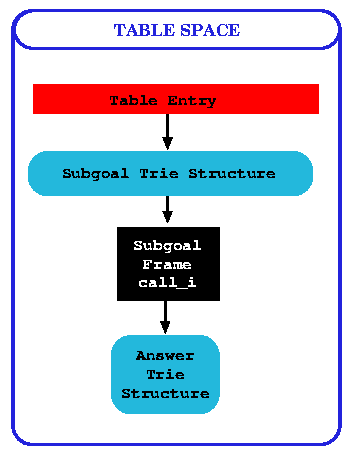
\includegraphics[scale=1.50]{\figs/table_space-0}}
\begin{lista}
  \item \lenitem{\redtext{Table Entry}: stores generic about the
    predicates.}
    \begin{sublista}
    \item \lenitem{\redtext{table} \yellowtext{predicate/2}.}
    \end{sublista}
\end{lista}

%%%%%%%%%%%%%%%%%%%%%%%%%%%%%%%%%%%%%%%%%%%%%%%%%%%%%%%%%%%%%%%%%%%%%%%%%%%
\titulo{Internal Table Space Architecture}

\mbox{}\hfill\raisebox{-\height}[0pt][0pt]{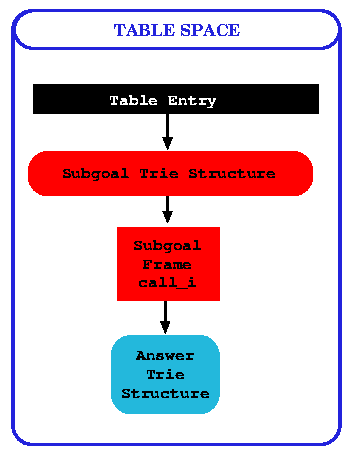
\includegraphics[scale=1.50]{\figs/table_space-1}}
\begin{lista}
  \item \lenitem{\redtext{Table Entry}: stores generic about the
    predicates.}
    \begin{sublista}
    \item \lenitem{\redtext{table} \yellowtext{predicate/2}.}
    \end{sublista}
  \item \lenitem{\redtext{Subgoal Trie Structure}: stores the
    \yellowtext{identifier} of the computations.}
    \begin{sublista}
    \item \lenitem{ \yellowtext{predicate}(\redtext{computation\_id}, Answer).}
    \end{sublista}
\end{lista}

%%%%%%%%%%%%%%%%%%%%%%%%%%%%%%%%%%%%%%%%%%%%%%%%%%%%%%%%%%%%%%%%%%%%%%%%%%%
\titulo{Internal Table Space Architecture}
\mbox{}\hfill\raisebox{-\height}[0pt][0pt]{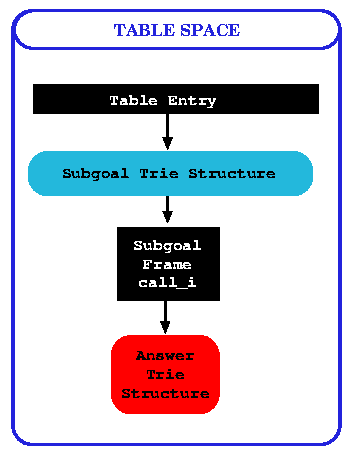
\includegraphics[scale=1.50]{\figs/table_space-2}}
\begin{lista}
  \item \lenitem{\redtext{Table Entry}: stores generic about the
    predicates.}
    \begin{sublista}
    \item \lenitem{\redtext{table} \yellowtext{predicate/2}.}
    \end{sublista}
  \item \lenitem{\redtext{Subgoal Trie Structure}: stores the
    \yellowtext{identifier} of the computations.}
    \begin{sublista}
    \item \lenitem{
      \yellowtext{predicate}(\redtext{computation\_id}, Answer).}
    \end{sublista}
  \item \lenitem{\redtext{Answer Trie Structure}: stores the
    \yellowtext{answers} of the computations.}
    \begin{sublista}
    \item \lenitem{\yellowtext{predicate}(computation\_id, \redtext{Answer}).}
   \end{sublista} 
\end{lista}

%%%%%%%%%%%%%%%%%%%% HERE

%%%%%%%%%%%%%%%%%%%%%%%%%%%%%%%%%%%%%%%%%%%%%%%%%%%%%%%%%%%%%%%%%%%%%%%%%%%
\titulo{Tabling Scheduling Strategies - Local vs Batched}

\vspace{-0.3in}
\begin{center}
  \multiinclude[format=pdf,graphics={scale=1.53}]{\figs/local_vs_batched}
\end{center}

%%%%%%%%%%%%%%%%%%%%%%%%%%%%%%%%%%%%%%%%%%%%%%%%%%%%%%%%%%%%%%%%%%%%%%%%%%%
\titulo{YapTab-Mt - Internal Architecture}

\vspace{-0.3in}
\begin{center}
  \multiinclude[format=pdf,graphics={scale=1.53}]{\figs/internal-arch}
\end{center}

%%%%%%%%%%%%%%%%%%%%%%%%%%%%%%%%%%%%%%%%%%%%%%%%%%%%%%%%%%%%%%%%%%%%%%%%%%%
\titulo{Private Answer Chaining - Key Idea}

\vspace{-0.3in}
\begin{center}
  \multiinclude[format=pdf,graphics={scale=1.53}]{\figs/pac_key_idea}
\end{center}


%%%%%%%%%%%%%%%%%%%%%%%%%%%%%%%%%%%%%%%%%%%%%%%%%%%%%%%%%%%%%%%%%%%%%%%%%%%
\titulo{Private Answer Chaining - Internals}


%%%%%%%%%%%%%%%%%%%%%%%%%%%%%%%%%%%%%%%%%%%%%%%%%%%%%%%%%%%%%%%%%%%%%%%%%%%
\titulo{Experimental Results - Worst Case Scenarios}
\begin{center}

\begin{tabular}{ll||cc|cc}
\multicolumn{2}{c||}{\multirow{2}{*}{\bf Threads}} &
\multicolumn{2}{c|}{\multirow{1}{*}{\bf NS}} &
\multicolumn{2}{|c}{\multirow{1}{*}{\bf FS}}\\ \cline{3-6}
& 
& \multicolumn{1}{c}{\yellowtext{Local}}
& \multicolumn{1}{c}{\yellowtext{Batched}}
& \multicolumn{1}{|c}{\yellowtext{Local}}
& \multicolumn{1}{c}{\yellowtext{Batched}}\\
\hline\hline
\multirow{4}{*}{\bf 1}
& \yellowtext{\bf Min }& \redtext{0.53}& 0.55& 1.01& \redtext{0.95}\\
& \yellowtext{\bf Avg }& \redtext{0.78}& 0.82& \redtext{1.30}& 1.46\\
& \yellowtext{\bf Max }& 1.06& \redtext{1.05}& \redtext{1.76}& 2.33\\
\hline
\multirow{4}{*}{\bf 8}
& \yellowtext{\bf Min }& 0.66& \redtext{0.63}& 1.16& \redtext{\bf  0.99}\\
& \yellowtext{\bf Avg }& \redtext{\bf 0.85}& 0.88& \redtext{\bf 1.88}& 1.95\\
& \yellowtext{\bf Max }& \redtext{\bf 1.12}& 1.14& \redtext{\bf 2.82}& 3.49\\
\hline
\multirow{4}{*}{\bf 16}
& \yellowtext{\bf Min }& 0.85& \redtext{0.75}& 1.17& \redtext{1.06}\\
& \yellowtext{\bf Avg }& \redtext{0.98}& 1.00& \redtext{1.97}& 2.08\\
& \yellowtext{\bf Max }& \redtext{1.16}& 1.31& \redtext{3.14}& 3.69\\
\hline
\multirow{4}{*}{\bf 24}
& \yellowtext{\bf Min }& \redtext{0.91}& 0.93& 1.16& \redtext{1.09}\\
& \yellowtext{\bf Avg }& \redtext{1.15}& 1.16& \redtext{2.06}& 2.19\\
& \yellowtext{\bf Max }& 1.72& \redtext{1.60}& \redtext{3.49}& 4.08\\
\hline
\multirow{4}{*}{\bf 32}
& \yellowtext{\bf Min }& 1.05& \redtext{1.04}& 1.33& \redtext{1.26}\\
& \yellowtext{\bf Avg }& 1.51& \redtext{1.49}& \redtext{2.24}& 2.41\\
& \yellowtext{\bf Max }& \redtext{2.52}& 2.63& \redtext{3.71}& 4.51\\
\end{tabular}
\end{center}

%%%%%%%%%%%%%%%%%%%%%%%%%%%%%%%%%%%%%%%%%%%%%%%%%%%%%%%%%%%%%%%%%%%%%%%%%%%

\titulo{Conclusions and Further Work}


%% %%%%%%%%%%%%%%%%%%%%%%%%%%%%%%%%%%%%%%%%%%%%%%%%%%%%%%%%%%%%%%%%%%%%%%%%%%%
%% \titulo{0-1 Knapsack Problem (Top-Down)}

%% \begin{lista}

%% \item An \yellowtext{item} is \yellowtext{included or excluded} from
%%   the \redtext{Knapsack} whether it \yellowtext{belongs or not} to the
%%   \yellowtext{best solution} of the problem.
%% \item Thread(s) scheduling:
%%   \begin{sublista}
%%   \item Threads \yellowtext{begin} their evaluation in the
%%     \yellowtext{top query}.
%% \item \yellowtext{Disperse threads} through the \yellowtext{evaluation
%%   tree} using \yellowtext{random branch orders}.
%%   \end{sublista}
%% \end{lista}

%% \begin{center}
%%   \multiinclude[format=pdf,graphics={width=26cm}]{\figs/top-down}
%% \end{center}

%% %%%%%%%%%%%%%%%%%%%%%%%%%%%%%%%%%%%%%%%%%%%%%%%%%%%%%%%%%%%%%%%%%%%%%%%%%%%

%% \titulo{0-1 Knapsack Problem (Bottom-Up)}

%% \begin{lista}
%% \item Evaluate the \yellowtext{combination} of \yellowtext{all items}
%%   with \yellowtext{all possible capacities} for the
%%   \redtext{Knapsack}. After all combinations are evaluated, the
%%   \yellowtext{best solution} of the problem has the \yellowtext{items
%%     that belong} to the \redtext{Knapsack}.

%% \item Thread(s) scheduling:
%%   \begin{sublista}
%%     \item \yellowtext{Divide} the \yellowtext{complete combination} in
%%       \yellowtext{smaller chunks} and \yellowtext{evaluate them} in
%%       the \yellowtext{threads}.
%%   \end{sublista}
%% \end{lista}

%% \begin{center}
%%   \multiinclude[format=pdf,graphics={width=26cm}]{\figs/bottom-up}
%% \end{center}

%% %%%%%%%%%%%%%%%%%%%%%%%%%%%%%%%%%%%%%%%%%%%%%%%%%%%%%%%%%%%%%%%%%%%%%%%%%%%
%% \titulo{Experimental Results - 0-1 Knapsack Problem}
%% \begin{center}
%% \begin{tabular}{cc||c|cccc|r}
%% \multicolumn{2}{c||}{\multirow{3}{*}{{\bf System/Dataset}}} 
%% & \multicolumn{6}{c}{{\bf \# Threads (p)}} \\ \cline{3-8}
%% & 
%% & {{\bf Time (T$_1$)}}  & \multicolumn{4}{c}{{\bf Speedup
%%     (T$_1$/T$_p$)}} & \multicolumn{1}{|c}{{\bf Best}}\\ 
%% & 
%% & {\bf 1} & {\bf 8} & {\bf 16} & {\bf 24} & {\bf 32} & {\bf Time}\\
%% \hline
%% \multicolumn{8}{l}{\yellowtext{Top-Down Approaches}} \\
%% \multicolumn{1}{c}{\multirow{3}{*} {\yellowtext{YAP$_{TD_1}$}}} 
%% & {\bf D$_{10}$} & 18,319 & 1.96 & \redtext{2.10} &      2.01  & 1.89 & 8,723 \\
%% & {\bf D$_{30}$} & 17,664 & 3.41 & \redtext{3.96} &      3.83  & 3.62 & 4,461 \\
%% & {\bf D$_{50}$} & 17,828 & 4.72 &      6.12  & \redtext{6.21} & 6.07 & 2,871 \\
%% \hline
%% \multicolumn{1}{c}{\multirow{3}{*} {\yellowtext{YAP$_{TD_2}$}}}
%% & {\bf D$_{10}$} & 23,816 & 6.78 & 11.95 & 14.81 & \redtext{16.79} & 1,418 \\
%% & {\bf D$_{30}$} & 25,049 & 7.39 & 13.63 & 16.85 & \redtext{19.35} & 1,295 \\
%% & {\bf D$_{50}$} & 24,866 & 7.38 & 13.67 & 16.78 & \redtext{19.23} & 1,293 \\
%% \hline
%% \multicolumn{8}{l}{\yellowtext{Bottom-Up Approaches}} \\
%% \multicolumn{1}{c}{\multirow{3}{*} {\yellowtext{YAP$_{BU}$}}}
%% & {\bf D$_{10}$} & 17,054 & 7.25 & 13.32 & 17.12 & \redtext{19.60} & 0,870\\
%% & {\bf D$_{30}$} & 17,005 & 7.22 & 13.47 & 17.29 & \redtext{19.64} & 0,866\\
%% & {\bf D$_{50}$} & 16,550 & 7.16 & 13.29 & 17.04 & \redtext{19.60} & 0,844\\
%% \hline
%% \multicolumn{1}{c}{\multirow{3}{*} {\yellowtext{XSB$_{BU}$}}} 
%% & {\bf D$_{10}$} & 37,338 & \redtext{0.81} & 0.79 & 0.73 & 0.54 & 37,338\\
%% & {\bf D$_{30}$} & 38,245 & \redtext{0.82} & 0.75 & 0.75 & 0.56 & 38,245\\
%% & {\bf D$_{50}$} & 39,100 & \redtext{0.82} & 0.79 & 0.73 & 0.54 & 39,100\\
%% \end{tabular}
%% \end{center}

%% %%%%%%%%%%%%%%%%%%%%%%%%%%%%%%%%%%%%%%%%%%%%%%%%%%%%%%%%%%%%%%%%%%%%%%%%%%%
%% \titulo{Experimental Results - LCS Problem}

%% \begin{center}
%% \begin{tabular}{cc||c|cccc|r}
%% \multicolumn{2}{c||}{\multirow{3}{*}{\bf System/Dataset}} 
%% & \multicolumn{6}{c}{\bf \# Threads (p)} \\ \cline{3-8}
%% & 
%% & {\bf Time (T$_1$)}  & \multicolumn{4}{c}{\bf Speedup (T$_1$/T$_p$)} 
%% & \multicolumn{1}{|c}{{\bf Best}}\\ 
%% & 
%% & {\bf 1} & {\bf 8} & {\bf 16} & {\bf 24} & {\bf 32} & {\bf Time} \\
%% \hline
%% \multicolumn{8}{l}{\yellowtext{Top-Down Approaches}} \\
%% \multicolumn{1}{c}{\multirow{3}{*}{\yellowtext{YAP$_{TD_1}$}}} 
%% & {\bf D$_{10}$} & 30,708 & \redtext{1.53} & 1.45 & 1.40 & 1.29 & 20,071 \\
%% & {\bf D$_{30}$} & 30,817 & \redtext{1.53} & 1.46 & 1.38 & 1.28 & 20,142 \\
%% & {\bf D$_{50}$} & 30,707 & \redtext{1.52} & 1.44 & 1.39 & 1.27 & 20,202 \\
%% \hline
%% \multicolumn{1}{c}{\multirow{3}{*}{\yellowtext{YAP$_{TD_2}$}}} 
%% & {\bf D$_{10}$} & 42,556 & 7.25 & 13.13 & 16.26 & \redtext{18.32} & 2,323 \\
%% & {\bf D$_{30}$} & 42,511 & 7.21 & 13.24 & 16.19 & \redtext{18.34} & 2,318 \\
%% & {\bf D$_{50}$} & 42,631 & 7.21 & 13.15 & 16.27 & \redtext{18.33} & 2,326 \\
%% \hline
%% \multicolumn{8}{l}{\yellowtext{Bottom-Up Approaches}} \\
%% \multicolumn{1}{c}{\multirow{3}{*}{\yellowtext{YAP$_{BU}$}}} 
%% & {\bf D$_{10}$} & 27,253 & 6.97 & 10.78 & 14.88 & \redtext{17.91} & 1,522 \\
%% & {\bf D$_{30}$} & 27,045 & 6.88 & 11.20 & 14.74 & \redtext{17.92} & 1,509 \\
%% & {\bf D$_{50}$} & 27,102 & 6.97 & 11.91 & 14.51 & \redtext{18.07} & 1,500 \\
%% \hline
%% \multicolumn{1}{c}{\multirow{3}{*}{\yellowtext{XSB$_{BU}$}}} 
%% & {\bf D$_{10}$} & 68,255 & n.a. & n.a. & n.a. & n.a. & 68,255\\
%% & {\bf D$_{30}$} & 69,700 & n.a. & n.a. & n.a. & n.a. & 69,700\\
%% & {\bf D$_{50}$} & 70,100 & n.a. & n.a. & n.a. & n.a. & 70,100\\
%% \end{tabular}

%% \end{center}

%% %%%%%%%%%%%%%%%%%%%%%%%%%%%%%%%%%%%%%%%%%%%%%%%%%%%%%%%%%%%%%%%%%%%%%%%%%%%

%% \titulo{Conclusions and Further Work}

%% \begin{lista}

%% \item The \redtext{0-1 Knapsack} and the \redtext{Longest Common
%%   Subsequence} problems are two well-know \yellowtext{dynamic
%%   programming problems}.
%%   \begin{sublista}
%%   \item We have \yellowtext{discussed} how we were able to
%%     \yellowtext{scale the execution} by taking advantage of the
%%     \redtext{YapTap-Mt} framework.
%%     \begin{sublista}  
%%       \item \redtext{Top-Down} vs \redtext{Bottom-Up}.
%%     \end{sublista}        
%%   \end{sublista} \pause
  
%% \item \yellowtext{Further work} will include:
%%   \begin{sublista}
%%     \item Use the \redtext{YapTap-Mt} framework in \yellowtext{other
%%       dynamic programming problems} and \yellowtext{domains}.
%%     \item Compare the \redtext{YapTap-Mt} framework with other
%%       \yellowtext{domain-specific languages} and \yellowtext{libraries
%%         for dynamic programming}.%%, such as \redtext{DPSKEL} %%or
%%       %%    \redtext{MALLBA}.
%%      \item Use \yellowtext{timestamped tries} to \yellowtext{reduce}
%%        even further the \yellowtext{memory used} in the table space.
%%   \end{sublista}
%% \end{lista}


%%%%%%%%%%%%%%%%%%%%%%%%%%%%%%%%%%%%%%%%%%%%%%%%%%%%%%%%%%%%%%%%%%%%%%%%%%%
\titulo{Research Outline}

\vspace{-0.3in}
\begin{center}
  \multiinclude[format=pdf,graphics={scale=1.10}]{\figs/work_stations}
\end{center}


%%%%%%%%%%%%%%%%%%%%%%%%%%%%%%%%%%%%%%%%%%%%%%%%%%%%%%%%%%%%%%%%%%%%%%%%%%%

\titulo{Thank You !!!}

%% \vspace{0.7cm}
%% \begin{center}
%% \animategraphics[width=23cm,autoplay,loop]{0.4}{\figs/thesis_tag_cloud-}{0}{3}

\end{document}




